\section{Introduction}
Software is becoming increasingly complex and at the same time increasingly safety critical.
Consider for example domains like robotics, autonomous systems such as cars, data-processing software, apps on mobile phones.
To tackle these challenges, developers need to reuse code and collaborate effectively.
Social coding platforms (\scp) comprise a number of so-called ecosystems i.e., large collections of interdependent software components that are maintained by large and geographically distributed communities of collaborating contributors~\cite{lungu:2008,decan:2017}. 
The ecosystems form large socio-technical networks of technical and social components that interact with each other on top of common software and hardware platforms.
The unprecedented growth of these ecosystems relies on substantial software reuse using different methods and tools \cite{mojica2014large}. 
\scp have substantially improved the situation on both the code reuse and collaboration, providing a huge bazaar of software and parts of software that can be reused through software repository forking and dependencies between projects; supported by the various facilities like pull requests, cross project traceabality, issue tracking systems (e.g. \texttt{JIRA}), source code reviews (e.g., \texttt{Gerrit}), Q\&A (e.g. \texttt{Stackoverflow}), continuous integration (e.g., \texttt{Travis CI}), and package distribution managers.




Forking a software repository produces distinct entities: a \textit{mainline} (i.e., the original repository) and several \textit{forked} repositories.
Two types of forks exist~\cite{Zhou:2020}: \textit{Social forks} are created for isolated development, but with the goal of contributing back to the mainline.
\textit{Variant forks} are created for splitting off a new development branch, often to steer the development into another direction than the mainline, without the intention to contribute back.
Variant forking may split the core development team and always splits the contributing community.
Variant forking creates variants of the mainline, which share common code, but also contain variant-specific code that needs to be maintained.
Such repositories represent families, inspired by the notion of \textit{software product lines}~\cite{berger.ea:2020:emse}.
The family members (consisting of mainline and one or more variant forks) are called \textbf{software variants} or products (a subset of software ecosystems).
They share common software artifacts as well as contain artifacts specific to one or multiple variants. 

\begin{figure}[ht]
  \begin{center}
  \small
  \vspace{-10pt}
    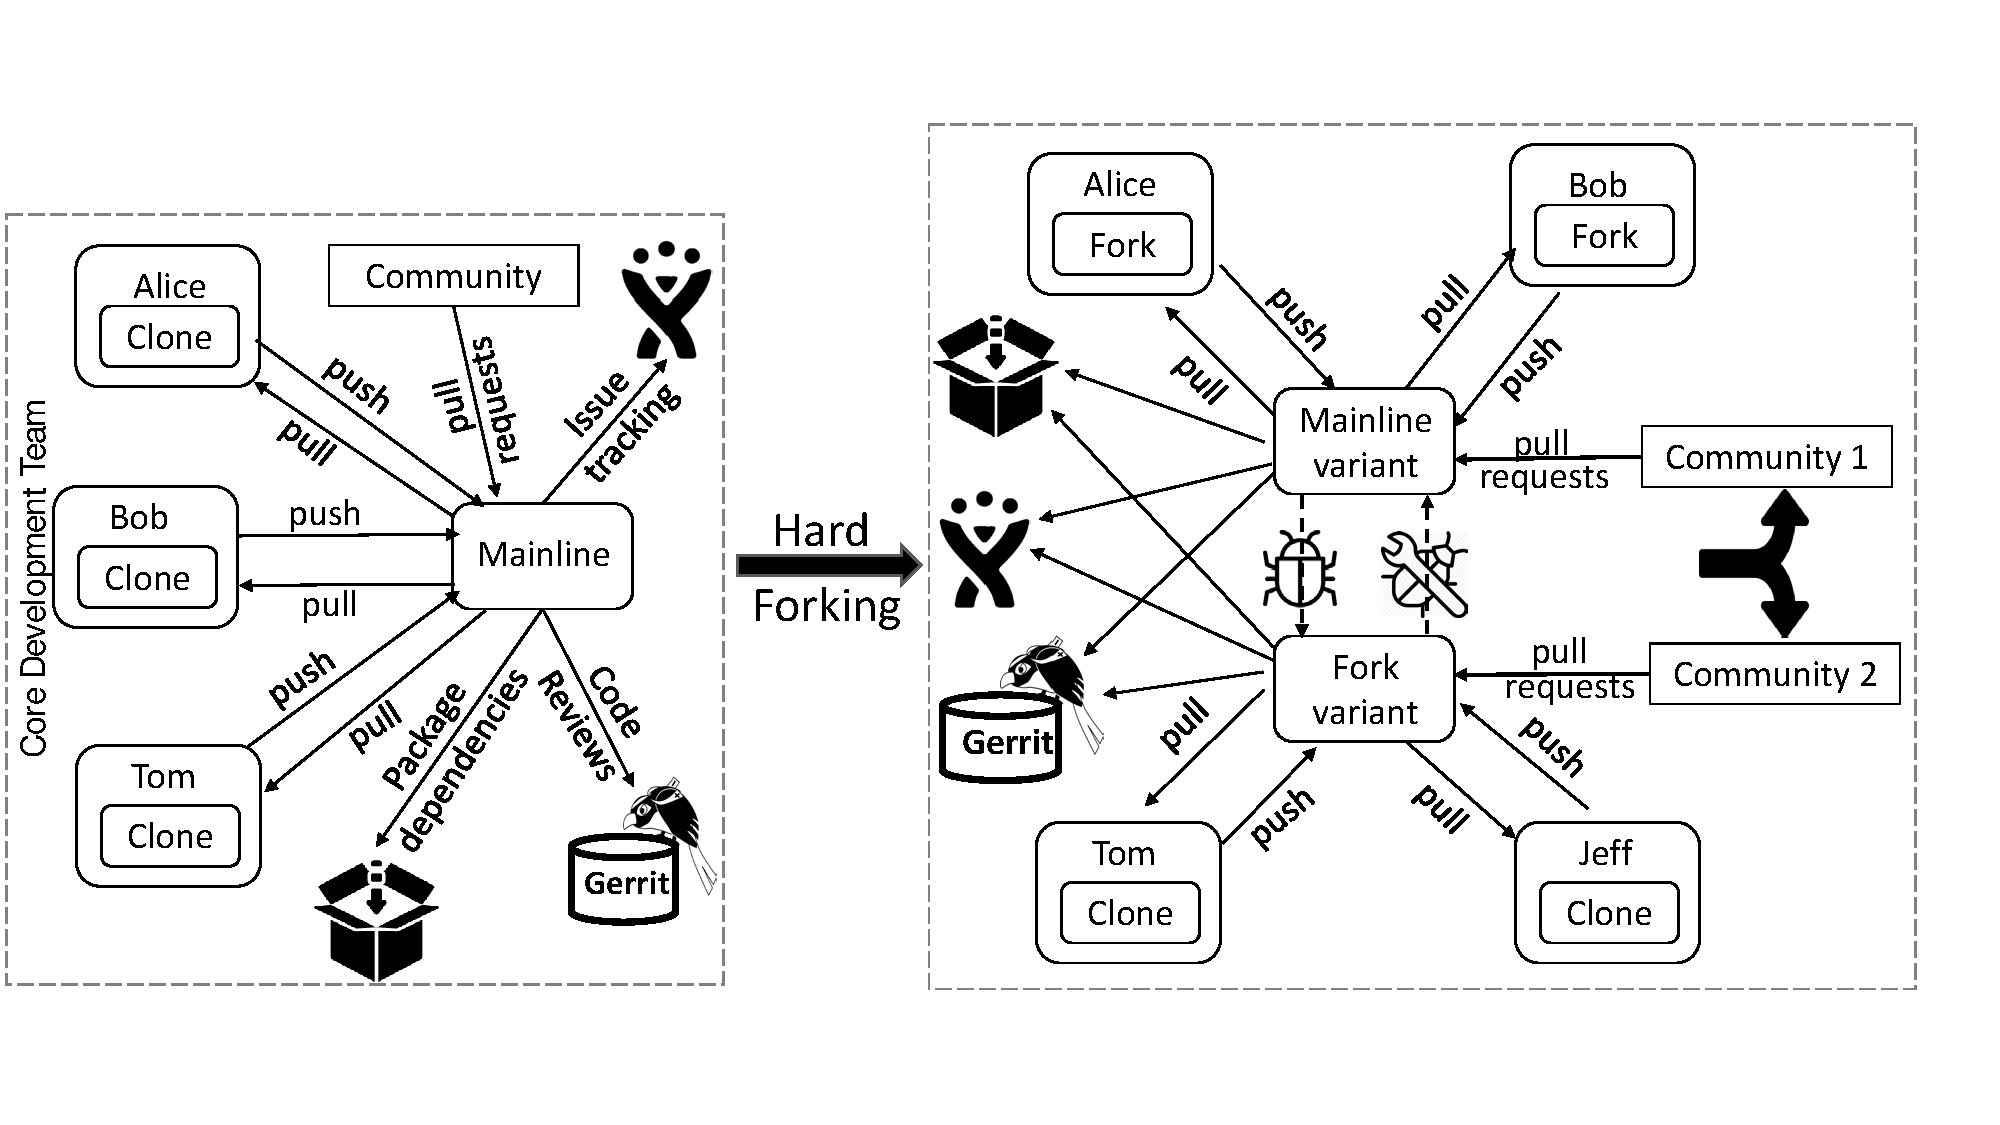
\includegraphics[width=0.5\textwidth]{figures/Collaboration.pdf}
  \end{center}
  \caption{Illustrating the maintenance of a repository before and after variant forking.}
  \vspace{-10pt}
  \label{fig:forking}
\end{figure}

In Figure~\ref{fig:forking} we present an illustration of a repository before and after variant forking. 
On the left part of the figure, we can see that there are three core developers: Alice, Bob and Tom who have write access to the mainline repository. 
The community interacts with the mainline through the following channels: sending pull requests, submitting issues and conducting change reviews. 
After variant forking, on the right part of the figure, the core developers are split into two. 
Alice and Bob remain with the mainline and Tom who is joined by a new developer Jeff starts maintaining a parallel project the fork variant. 
As can be seen, the parallel projects mainline and variant have split the contributing community. New contributors could decide to contribute to mainline or variant, for instance depending on the one which is more accommodative to contributions.
Furthermore, as a result of parallel maintenance, developers in one of the projects may identify and fix bugs in shared artifacts. 
These fixes could be propagated to other members of the family to avoid effort duplication.

Many studies have researched on variant forks; however, most of these studies were carried out in the pre-\scp days of \texttt{SourceForge}, before the advent of social coding environment~\cite{Linus:2012Perspectives,Gregorio:2012,Viseur:2012Forks,Linus:2013CodeForking,Laurent:2008,Linus:2011ToFork}. 
We have found only two studies that have investigated variant forks on \gh~\cite{businge2018appfamilies,Zhou:2020}.  
While studies report controversial perceptions around hard forks in the pre-\gh days~\cite{Chua:Forking:2017,Dixion:2009Forks,Ernst:2010,Linus:2011ToFork,Linus:2014Hackers,Raymond:Cathedral:2001}, Zhou et al.~\cite{Zhou:2020} report that these perceptions have changed with the advent of \gh. Jiang et al.~\cite{Lo:2017} state that, although forking is controversial in traditional open source software (OSS) community, it is encouraged and is a built-in feature in \gh. Jiang et al. ~\cite{Lo:2017} further report that developers fork repositories to submit pull requests, fix bugs, add new features and keep copies (social forks). 
Zhou et al.~\cite{Zhou:2020} also report that most variant forks start as social forks. 

While numerous studies have investigated variant forking, we do not know any study that has investigated the socio-technical specificities of these variant forks. 
Our research aims at empirically studying the evolution of \textbf{software families} by investigating their socio-technical aspects. 
For the social aspects, it would be interesting to look at the interaction and collaboration between communities involved in the mainline and variants.
How different are collaborations with respect to who forked and how the fork has been created?
For the technical aspects, as an example, considering the dependent packages, it would be interesting to investigate if developers migrate from one variant of the required package to another in a family.
As preliminary steps, in this paper we investigate the socio-tachnical aspects of forking in the large ecosystem of \js \np packages. More specifically, we focus on three research questions:
\begin{itemize}
\item[\textbf{RQ0}] \textit{How prevalent are software families in software ecosystems?} 
This question will help us determine whether the research goal is worthwhile to pursue: if software families rarely exist, results about their social-technical evolution may not be statistically significant.  

\item[\textbf{RQ1}] \textit{How does the distribution on package releases of mainlines and their variants compare to each other? }
This RQ will help us determine if mainlines and variants are continuously maintained. 
Do most variants have one-off releases?

\item[\textbf{RQ2}] \textit{How does the distribution on package dependencies of mainlines and their variants compare to each other?}
This RQ will help us determine if members in the software families depend on other packages in the \np ecosystem.

\item[\textbf{RQ3}] \textit{Do the variant projects have dependent packages\,/\,projects?}
This research question will help us determine other packages\,/\,projects in the ecosystem that depend on the variant projects.
Since they are forks of the mainline, it would be interesting to find some variants that have more dependent packages\,/\,projects.
\end{itemize}

